%%%%%%%%%%%%%%%%%%%%%%%%%%%%%%%%%%%%%%%%%%%%%%%%%%%%%%%%%%%%%%%%%%%
%                                                                 %
%  GEANT manual in LaTeX form                              %
%                                                                 %
%  Michel Goossens (for translation into LaTeX)                   %
%  Version 1.00                                                   %
%  Last Mod. Jan 24 1991  1300   MG + IB                          %
%                                                                 %
%%%%%%%%%%%%%%%%%%%%%%%%%%%%%%%%%%%%%%%%%%%%%%%%%%%%%%%%%%%%%%%%%%%
\Origin{R.Brun, A.McPherson}
\Submitted{15.08.83}            \Revised{08.11.93}
\Version{Geant 3.16}\Routid{GEOM050}
\Makehead{The GEANT shapes}
 
The {\tt GEANT} geometry package offers sixteen basic shapes with which
to describe the setups where particles are transported. In this section
we will describe these shapes. For each shape figs~(\ref{fg:geom050-1}),
(\ref{fg:geom050-2}), (\ref{fg:geom050-3}), (\ref{fg:geom050-4}) 
show a simple drawing illustrating the
meaning of the parameters and the position and orientation of the
reference frame proper of that shape. A description of the shapes and of
their parameters follows. Angles are always in degrees. With every shape is
given the code which is used internally by {\tt GEANT} to identify it.
 
\begin{DLtt}{MMMMMMMM}
\item[1  BOX] box with faces perpendicular to the
axes. It has 3 parameters:
\begin{enumerate}
\item {\tt DX} half-length of the box along the x-axis;
\item {\tt DY} half-length of the box along the y-axis;
\item {\tt DZ} half-length of the box along the z-axis;
\end{enumerate}
 
\item[2  TRD1] trapezoid with the x dimension varying along z. It has
4 parameters:
\begin{enumerate}
\item {\tt DX1} half-length along x at the z surface positioned
at {\tt -DZ};
\item {\tt DX2} half-length along x at the z surface positioned
at {\tt +DZ};
\item {\tt DY} half-length along the y-axis;
\item {\tt DZ} half-length along the z-axis;
\end{enumerate}
 
\item[3  TRD2] trapezoid with both x and y dimensions varying along z.
It has 5 parameters:
\begin{enumerate}
\item {\tt DX1} half-length along x at the z surface positioned
at {\tt -DZ};
\item {\tt DX2} half-length along x at the z surface positioned
at {\tt +DZ};
\item {\tt DY1} half-length along y at the z surface positioned
at {\tt -DZ};
\item {\tt DY2} half-length along y at the z surface positioned
at {\tt +DZ};
\item {\tt DZ} half-length along the z-axis;
\end{enumerate}

\item[4  TRAP] {\it general} trapezoid: the
faces perpendicular to z are trapezia and their centres are not necessarily
on a line parallel to the z axis. This shape has 11 parameters, but only 
considering that the faces should be planar, only 9 are really independent.
A check is performed on the user parameters and a message is printed in
case of non-planar faces. Ignoring this warning may cause unpredictable
effect at tracking time.
\begin{enumerate}
\item {\tt DZ} half-length along the z axis;
\item {\tt THET} polar angle of the line joining the centre of the
face at {\tt -DZ} to the centre of the one at {\tt +DZ};
\item {\tt PHI} azimuthal angle of the line joining the centre of the
face at {\tt -DZ} to the centre of the one at {\tt +DZ};
\item {\tt H1} half-length along y of the face at {\tt -DZ};
\item {\tt BL1} half-length along x of the side at {\tt -H1}
in y of the face at {\tt -DZ} in z;
\item {\tt TL1} half-length along x of the side at {\tt +H1}
in y of the face at {\tt -DZ} in z;
\item {\tt ALP1} angle with respect to the y axis from the centre
of the side at {\tt -H1} in y to the centre 
of the side at {\tt +H1} in y of the face at {\tt -DZ} in z;
\item {\tt H2} half-length along y of the face at {\tt +DZ};
\item {\tt BL2} half-length along x of the side at {\tt -H2}
in y of the face at {\tt +DZ} in z;
\item {\tt TL2} half-length along x of the side at {\tt +H2}
in y of the face at {\tt +DZ} in z;
\item {\tt ALP2} angle with respect to the y axis from the centre
of the side at {\tt -H2} in y to the centre 
of the side at {\tt +H2} in y of the face at {\tt +DZ} in z;
\end{enumerate}
 
\item[5  TUBE] tube. It has 3 parameters:
\begin{enumerate}
\item {\tt RMIN} inside radius;
\item {\tt RMAX} outside radius;
\item {\tt DZ} half length in z;
\end{enumerate}

\item[6  TUBS] $\phi$ segment of a tube. It has 5 parameters:
\begin{enumerate}
\item {\tt RMIN} inside radius;
\item {\tt RMAX} outside radius;
\item {\tt DZ} half length in z;
\item {\tt PHI1} starting angle of the segment;
\item {\tt PHI2} ending angle of the segment;
\end{enumerate}
{\tt PHI1} should be smaller than {\tt PHI2}. If this is not the case,
the system adds 360 degrees to {\tt PHI2}.
 
\item[7  CONE] conical tube. It has 5 parameters:
\begin{enumerate}
\item {\tt DZ} half-length in z;
\item {\tt RMN1} inside radius at {\tt -DZ} in z;
\item {\tt RMX1} outside radius at {\tt -DZ} in z;
\item {\tt RMN2} inside radius at {\tt +DZ} in z;
\item {\tt RMX2} outside radius at {\tt +DZ} in z;
\end{enumerate}

 
\item[8  CONS] $\phi$ segment of a conical tube. It has 7 parameters:
\begin{enumerate}
\item {\tt DZ} half-length in z;
\item {\tt RMN1} inside radius at {\tt -DZ} in z;
\item {\tt RMX1} outside radius at {\tt -DZ} in z;
\item {\tt RMN2} inside radius at {\tt +DZ} in z;
\item {\tt RMX2} outside radius at {\tt +DZ} in z;
\item {\tt PHI1} starting angle of the segment;
\item {\tt PHI2} ending angle of the segment;
\end{enumerate}
{\tt PHI1} should be smaller than {\tt PHI2}. If this is not the case,
the system adds 360 degrees to {\tt PHI2}.

\item[9  SPHE] segment of spherical shell. It has 6 parameters:
\begin{enumerate}
\item {\tt RMIN} inside radius of the shell;
\item {\tt RMAX} outside radius of the shell;
\item {\tt THE1} starting polar angle of the shell;
\item {\tt THE2} ending polar angle of the shell;
\item {\tt PHI1} starting azimuthal angle of the shell;
\item {\tt PHI2} ending azimuthal angle of the shell;
\end{enumerate}
 
\item[10  PARA] parallelepiped. It has 6 parameters:
\begin{enumerate}
\item {\tt DX} half-length in x;
\item {\tt DY} half-length in y;
\item {\tt DZ} half-length in z;
\item {\tt ALPH} angle formed by the y axis and by the plane joining the
centre of the faces parallel to the z-x plane at {\tt -DY} and {\tt +DY};
\item {\tt THET} polar angle of the line joining the centres of the faces
at {\tt -DZ} and {\tt +DZ} in z;
\item {\tt PHI} azimuthal angle of the line joining the centres of the faces
at {\tt -DZ} and {\tt +DZ} in z;
\end{enumerate}

\item[11  PGON] {\it polygon}. It has at least 10 parameters:
\begin{enumerate}
\item {\tt PHI1} the azimuthal angle $\phi$ at which the volume {\it begins}
(angles are counted counterclockwise);
\item {\tt DPHI} {\it opening} angle of the volume, which extends from
{\tt PHI1} to {\tt PHI1+DPHI};
\item {\tt NPDV} number of sides of the cross section between the
given $\phi$ limits;
\item {\tt NZ} number of planes perpendicular to the z axis where the
dimension of the section is given -- this number should be at least
2 and {\tt NP} triplets of numbers must follow;
\item {\tt Z} z coordinate of the section;
\item {\tt RMIN} radius of the circle tangent to the sides of the inner
polygon in the cross-section;
\item {\tt RMAX} radius of the circle tangent to the sides of the outer
polygon in the cross-section;
\end{enumerate}

\item[12  PCON] {\it polycone}. It has at least 9 parameters:
\begin{enumerate}
\item {\tt PHI1} the azimuthal angle $\phi$ at which the volume {\it begins}
(angles are counted counterclockwise);
\item {\tt DPHI} {\it opening} angle of the volume, which extends from
{\tt PHI1} to {\tt PHI1+DPHI};
\item {\tt NZ} number of planes perpendicular to the z axis where the
dimension of the section is given -- this number should be at least
2 and {\tt NP} triplets of numbers must follow;
\item {\tt Z} z coordinate of the section;
\item {\tt RMIN} radius of the inner circle in the cross-section;
\item {\tt RMAX} radius of the outer circle in the cross-section;
\end{enumerate}

\item[13 ELTU] elliptical cross-section tube. It has three parameters:
\begin{enumerate}
\item {\tt P1} semi-axis of the ellipse along x;
\item {\tt P2} semi-axis of the ellipse along y;
\item {\tt DZ} half-length in z;
\end{enumerate}

The equation of the surface is $x^2\mbox{\tt P1}^{-2} + y^2
\mbox{\tt P2}^{-2} = 1$.

\item[14 HYPE] hyperbolic  tube, i.e. the inner and  outer surfaces are
hyperboloids, as would be formed by a system of cylindrical
wires  which were  then  rotated  tangentially about  their
centres. It has  4  parameters:
\begin{enumerate}
\item {\tt RMIN} inner radius at z=0, where tube is narrowest;
\item {\tt RMAX} outer radius at z=0, where tube is narrowest;
\item {\tt DZ} half-length in z;
\item {\tt THET} {\it stereo  angle} of rotation of the two faces;
\end{enumerate}

The hyperbolic  surfaces are  given by: $r^2 = (z \tan \theta )^2
+r_{z=0}^2$

\item[28  GTRA] general twisted trapezoid: the
faces perpendicular to z are trapezia and their centres are not necessarily
on a line parallel to the z axis as the {\tt TRAP}; additionally, the
faces may be {\it twisted} so that none of their edges are parallel. 
It is a {\tt TRAP} shape, except that it is {\it twisted}
in the x-y plane as a function of z. 
The parallel sides perpendicular to the z axis
are rotated with respect to the x axis by an angle {\tt
TWIST}, which is one of the parameters. The shape is defined by the eight
corners and is assumed to be constructed of straight lines joining points on
the boundary of the trapezoidal face at z=-DZ to the corresponding points on the
face at z=DZ. Divisions are not allowed.  It has 12 parameters: 
\begin{enumerate}
\item {\tt DZ} half-length along the z axis;
\item {\tt THET} polar angle of the line joining the centre of the
face at {\tt -DZ} to the centre of the one at {\tt +DZ};
\item {\tt PHI} azimuthal angle of the line joining the centre of the
face at {\tt -DZ} to the centre of the one at {\tt +DZ};
\item {\tt TWIST} {\it twist} angle of the faces parallel to the x-y plane
at z = $\pm${\tt DZ} around an axis parallel to z passing through their
centre;
\item {\tt H1} half-length along y of the face at {\tt -DZ};
\item {\tt BL1} half-length along x of the side at {\tt -H1}
in y of the face at {\tt -DZ} in z;
\item {\tt TL1} half-length along x of the side at {\tt +H1}
in y of the face at {\tt -DZ} in z;
\item {\tt ALP1} angle with respect to the y axis from the centre
of the side at {\tt -H1} in y to the centre 
of the side at {\tt +H1} in y of the face at {\tt -DZ} in z;
\item {\tt H2} half-length along y of the face at {\tt +DZ};
\item {\tt BL2} half-length along x of the side at {\tt -H2}
in y of the face at {\tt +DZ} in z;
\item {\tt TL2} half-length along x of the side at {\tt +H2}
in y of the face at {\tt +DZ} in z;
\item {\tt ALP2} angle with respect to the y axis from the centre
of the side at {\tt -H2} in y to the centre 
of the side at {\tt +H2} in y of the face at {\tt +DZ} in z;
\end{enumerate}

{\bf Note:} this shape suffers from the same limitations than the {\tt TRAP}:
the tracking routines assume that the faces are planar, but this constraint
is not easily expressed in terms of the 12 parameters. Additionally, no check
on the faces is performed in this case. Users should avoid to use this shape
as much as possible, and if they have to do so, they should make sure that the
faces are really planes. If this is not the case, the result of the transport
is unpredictable.

To accelerate the computations necessary for transport, 18 additional 
parameters are calculated for this shape:

\begin{enumerate}
\item {\tt DX0DZ} $dx/dz$ of the line joining the centres of the faces at 
z=$\pm${\tt DZ};
\item {\tt DY0DZ} $dy/dz$ of the line joining the centres of the faces at 
z=$\pm${\tt DZ};
\item {\tt X01} x at z=0 for line joining the
+ on parallel side, perpendicular corners at z=$\pm${\tt DZ};
\item {\tt Y01} y at z=0 for line joining the
+ on parallel side, + on perpendicular corners at z=$\pm${\tt DZ};
\item {\tt DXDZ1} $dx/dz$ for line joining the + on parallel side,
+ on perpendicular corners at z=$\pm${\tt DZ};
\item {\tt DYDZ1} $dy/dz$ for line joining the + on parallel side,
+ on perpendicular corners at z=$\pm${\tt DZ};
\item {\tt X02} x at z=0 for line joining the - on parallel side,
+ on perpendicular corners at z=$\pm${\tt DZ};
\item {\tt Y02} y at z=0 for line joining the - on parallel side,
+ on perpendicular corners at z=$\pm${\tt DZ};
\item {\tt DXDZ2} $dx/dz$ for line joining the - on parallel side,
+ on perpendicular corners at z=$\pm${\tt DZ};
\item {\tt DYDZ2} $dy/dz$ for line joining the - on parallel side, 
+ on perpendicular corners at z=$\pm${\tt DZ};
\item {\tt X03} x at z=0 for line joining the - on parallel side,
- on perpendicular corners at z=$\pm${\tt DZ};
\item {\tt Y03} y at z=0 for line joining the - on parallel side,
- on perpendicular corners at z=$\pm${\tt DZ};
\item {\tt DXDZ3} $dx/dz$ for line joining the - on parallel side,
- on perpendicular corners at z=$\pm${\tt DZ};
\item {\tt DYDZ3} $dy/dz$ for line joining the - on parallel side,
- on perpendicular corners at z=$\pm${\tt DZ};
\item {\tt X04} x at z=0 for line joining the + on parallel side,
- on perpendicular corners at z=$\pm${\tt DZ};
\item {\tt Y04} y at z=0 for line joining the + on parallel side,
- on perpendicular corners at z=$\pm${\tt DZ};
\item {\tt DXDZ4} $dx/dz$ for line joining the + on parallel side,
- on perpendicular corners at z=$\pm${\tt DZ};
\item {\tt DYDZ4} $dy/dz$ for line joining the + on parallel side,
- on perpendicular corners at z=$\pm${\tt DZ};
\end{enumerate}

\item[29 CTUB] {\it cut} tube, a tube cut at the extremities with planes
not necessarily perpendicular to the z axis. It has 11 parameters:
\begin{enumerate}
\item {\tt RMIN} inside radius;
\item {\tt RMAX} outside radius;
\item {\tt DZ} half length in z;
\item {\tt PHI1} starting angle of the segment;
\item {\tt PHI2} ending angle of the segment;
\item {\tt LX} x component of a unit vector perpendicular to the face at {\tt -DZ};
\item {\tt LY} y component of a unit vector perpendicular to the face at {\tt -DZ};
\item {\tt LZ} z component of a unit vector perpendicular to the face at {\tt -DZ};
\item {\tt HX} x component of a unit vector perpendicular to the face at {\tt +DZ};
\item {\tt HY} y component of a unit vector perpendicular to the face at {\tt +DZ};
\item {\tt HZ} z component of a unit vector perpendicular to the face at {\tt +DZ};
\end{enumerate}
{\tt PHI1} should be smaller than {\tt PHI2}. If this is not the case,
the system adds 360 degrees to {\tt PHI2}.
\end{DLtt}
\newpage
\begin{figure}[hbt]
\vspace{3cm}
      \centering
      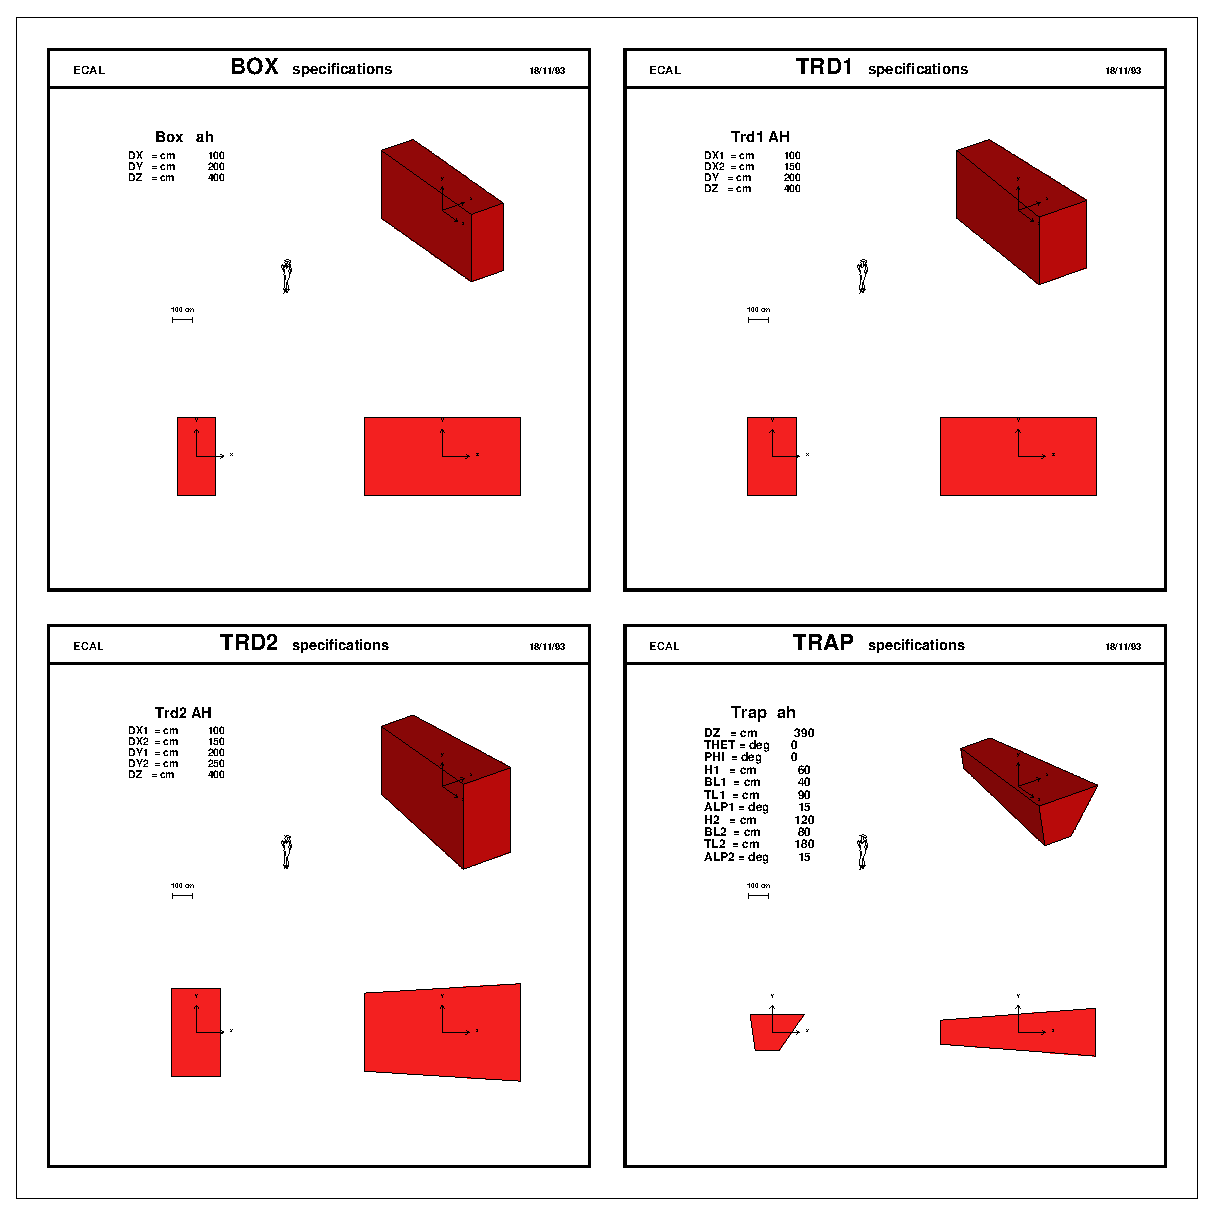
\epsfig{file=eps/geom050-1.eps,width=16cm}
      \caption{shapes {\tt BOX, TRD1, TRD2, TRAP}}
      \label{fg:geom050-1}
\end{figure}
\newpage
\begin{figure}[hbt]
\vspace{3cm}
      \centering
      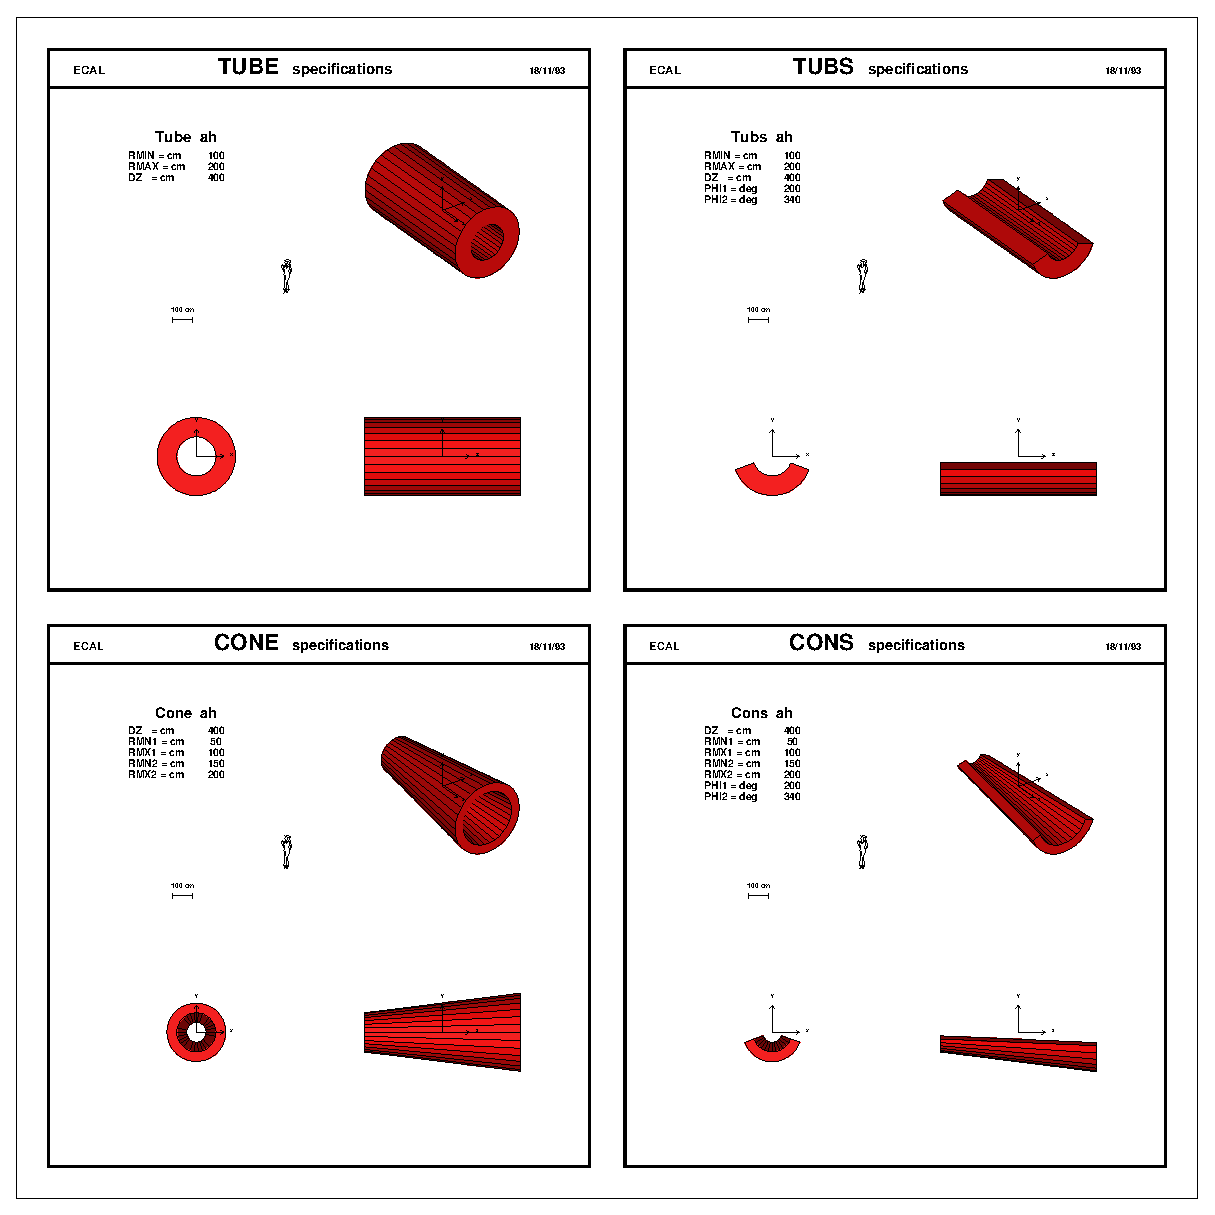
\epsfig{file=eps/geom050-2.eps,width=16cm}
      \caption{shapes {\tt TUBE, TUBS, CONE, CONS}}
      \label{fg:geom050-2}
\end{figure}
\newpage
\begin{figure}[hbt]
\vspace{3cm}
      \centering
      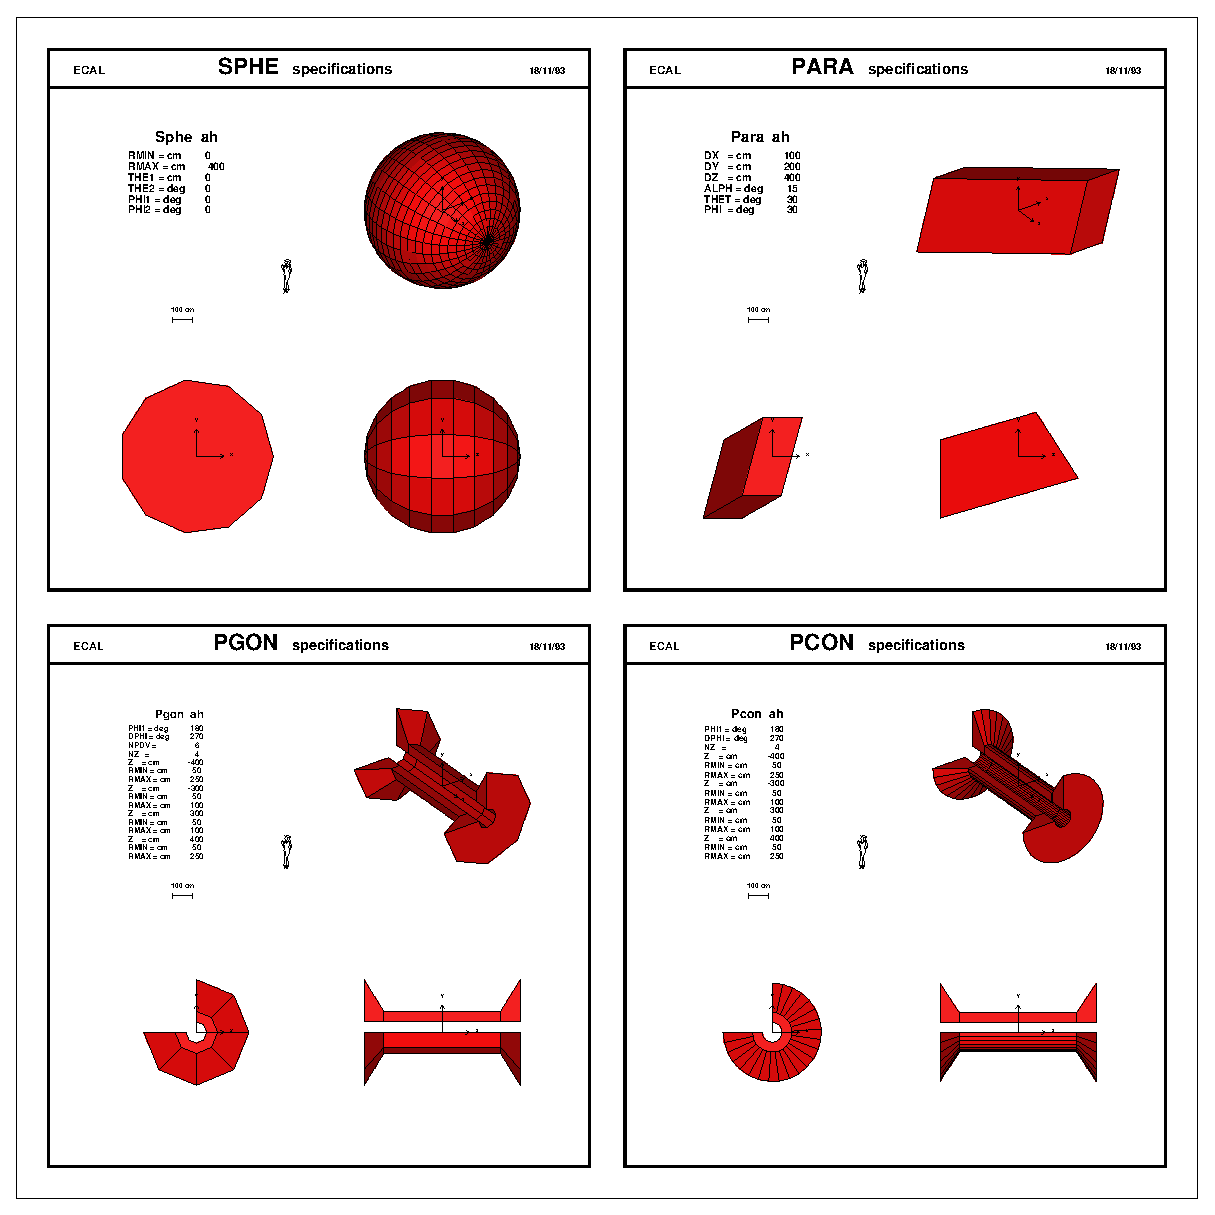
\epsfig{file=eps/geom050-3.eps,width=16cm}
      \caption{shapes {\tt PARA, SPHE, PGON, PCON}}
      \label{fg:geom050-3}
\end{figure}
\newpage
\begin{figure}[hbt]
\vspace{3cm}
      \centering
      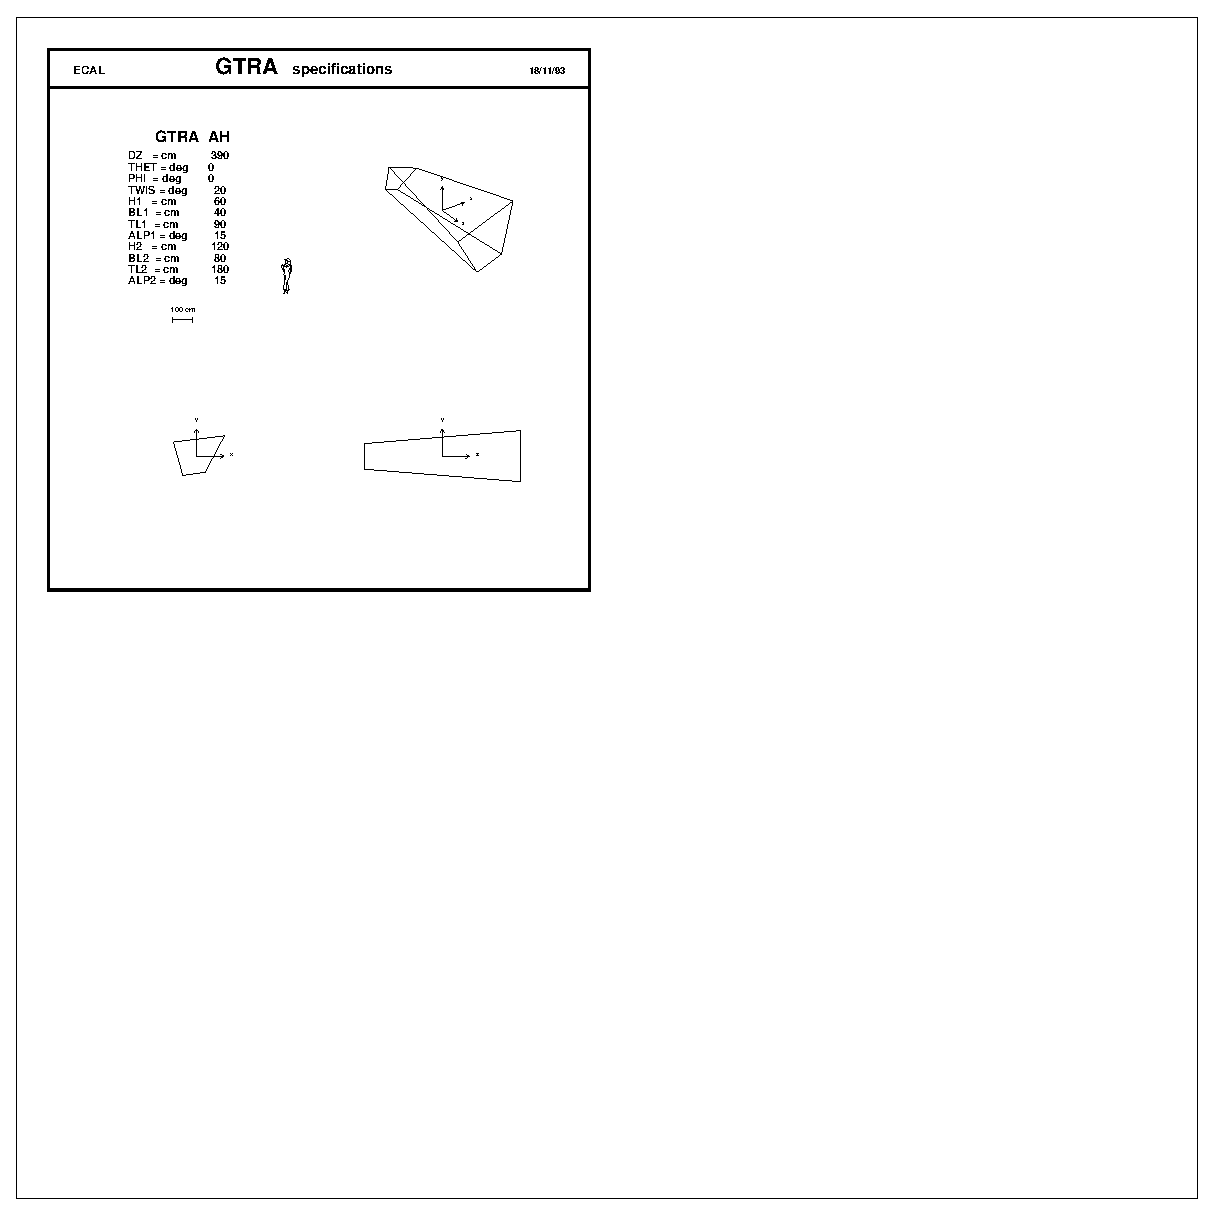
\epsfig{file=eps/geom050-4.eps,width=16cm}
      \caption{shapes {\tt GTRA}}
      \label{fg:geom050-4}
\end{figure}
